% -*- TeX-engine: xetex; eval: (auto-fill-mode 0); eval: (visual-line-mode 1); -*-
% Compile with XeLaTeX

%%%%%%%%%%%%%%%%%%%%%%%
% Option 1: Slides: (comment for handouts)   %
%%%%%%%%%%%%%%%%%%%%%%%

\documentclass[slidestop,compress,mathserif,12pt,t,professionalfonts,xcolor=table]{beamer}

% solution stuff
\newcommand{\solnMult}[1]{
\only<1>{#1}
\only<2->{\red{\textbf{#1}}}
}
\newcommand{\soln}[1]{\textit{#1}}

%%%%%%%%%%%%%%%%%%%%%%%%%%%%%%%
% Option 2: Handouts, without solutions (post before class)    %
%%%%%%%%%%%%%%%%%%%%%%%%%%%%%%%

% \documentclass[11pt,containsverbatim,handout,xcolor=xelatex,dvipsnames,table]{beamer}

% % handout layout
% \usepackage{pgfpages}
% \pgfpagesuselayout{4 on 1}[letterpaper,landscape,border shrink=5mm]

% % solution stuff
% \newcommand{\solnMult}[1]{#1}
% \newcommand{\soln}[1]{}

%%%%%%%%%%%%%%%%%%%%%%%%%%%%%%%%%%%%
% Option 3: Handouts, with solutions (may post after class if need be)    %
%%%%%%%%%%%%%%%%%%%%%%%%%%%%%%%%%%%%

% \documentclass[11pt,containsverbatim,handout,xcolor=xelatex,dvipsnames,table]{beamer}

% % handout layout
% \usepackage{pgfpages}
% \pgfpagesuselayout{4 on 1}[letterpaper,landscape,border shrink=5mm]

% % solution stuff
% \newcommand{\solnMult}[1]{\red{\textbf{#1}}}
% \newcommand{\soln}[1]{\textit{#1}}

%%%%%%%%%%
% Load style file, defaults  %
%%%%%%%%%%

%%%%%%%%%%%%%%%%
% Themes
%%%%%%%%%%%%%%%%

% See http://deic.uab.es/~iblanes/beamer_gallery/ for mor options

% Style theme
\usetheme{metropolis}

% Color theme
%\usecolortheme{seahorse}

% Helvetica Neue Light for most text
%\usepackage{fontspec}
%\setsansfont{Helvetica Neue Light}

%%%%%%%%%%%%%%%%
% Packages
%%%%%%%%%%%%%%%%

\usepackage{geometry}
\usepackage{graphicx}
\usepackage{amssymb}
\usepackage{epstopdf}
\usepackage{amsmath}  	% this permits text in eqnarray among other benefits
\usepackage{url}		% produces hyperlinks
\usepackage[english]{babel}
\usepackage{colortbl}	% allows for color usage in tables
\usepackage{multirow}	% allows for rows that span multiple rows in tables
\usepackage{color}		% this package has a variety of color options
\usepackage{pgf}
\usepackage{calc}
\usepackage{ulem}
\usepackage{multicol}
\usepackage{textcomp}
\usepackage{listings}
\usepackage{changepage}
\usepackage{tikz}
\usetikzlibrary{trees}		% for probability trees
\usepackage{fancyvrb}	% for colored code chunks
\usepackage{nameref}

%%%%%%%%%%%%%%%%
% Remove navigation symbols
%%%%%%%%%%%%%%%%

\beamertemplatenavigationsymbolsempty
\hypersetup{pdfpagemode=UseNone} % don't show bookmarks on initial view

%%%%%%%%%%%%%%%%
% User defined colors
%%%%%%%%%%%%%%%%

% Pantone 2016 Spring colors
% https://atelierbram.github.io/c-tiles16/colorscheming/pantone-spring-2016-colortable.html
% update each semester or year

\xdefinecolor{custom_blue}{rgb}{0.01, 0.31, 0.52} % Snorkel Blue
\xdefinecolor{custom_darkBlue}{rgb}{0.20, 0.20, 0.39} % Reflecting Pond  
\xdefinecolor{custom_orange}{rgb}{0.96, 0.57, 0.42} % Cadmium Orange
\xdefinecolor{custom_green}{rgb}{0, 0.47, 0.52} % Biscay Bay
\xdefinecolor{custom_red}{rgb}{0.58, 0.32, 0.32} % Marsala

\xdefinecolor{custom_lightGray}{rgb}{0.78, 0.80, 0.80} % Glacier Gray
\xdefinecolor{custom_darkGray}{rgb}{0.35, 0.39, 0.43} % Stormy Weather

%%%%%%%%%%%%%%%%
% Template colors
%%%%%%%%%%%%%%%%

%\setbeamercolor*{palette primary}{fg=white,bg= custom_blue}
%\setbeamercolor*{palette secondary}{fg=black,bg= custom_blue!80!black}
%\setbeamercolor*{palette tertiary}{fg=white,bg= custom_blue!80!black!80}
%\setbeamercolor*{palette quaternary}{fg=white,bg= custom_blue}
%
%\setbeamercolor{structure}{fg= custom_blue}
%\setbeamercolor{frametitle}{bg= custom_blue!90}
%\setbeamertemplate{blocks}[shadow=false]
%\setbeamersize{text margin left=2em,text margin right=2em}

%%%%%%%%%%%%%%%%
% Styling fonts, bullets, etc.
%%%%%%%%%%%%%%%%
%
%% title slide
%\setbeamerfont{title}{size=\large,series=\bfseries}
%\setbeamerfont{subtitle}{size=\large,series=\mdseries}
%%\setbeamerfont{institute}{size=\large,series=\mdseries}
%
% color of alerted text
\setbeamercolor{alerted text}{fg=custom_orange}

% styling of itemize bullets
\setbeamercolor{item}{fg=custom_blue}
\setbeamertemplate{itemize item}{{{\small$\blacktriangleright$}}}
\setbeamercolor{subitem}{fg=custom_blue}
\setbeamertemplate{itemize subitem}{{\textendash}}
\setbeamerfont{itemize/enumerate subbody}{size=\footnotesize}
\setbeamerfont{itemize/enumerate subitem}{size=\footnotesize}

% styling of enumerate bullets
\setbeamertemplate{enumerate item}{\insertenumlabel.}

%\setbeamerfont{enumerate item}{family={\fontspec{Helvetica Neue}}}
%\setbeamerfont{enumerate subitem}{family={\fontspec{Helvetica Neue}}}
%\setbeamerfont{enumerate subsubitem}{family={\fontspec{Helvetica Neue}}}

% make frame titles small to make room in the slide
\setbeamerfont{frametitle}{size=\small} 




%% set Helvetica Neue font for frame and section titles
%\setbeamerfont{frametitle}{family={\fontspec{Helvetica Neue}}}
%\setbeamerfont{sectiontitle}{family={\fontspec{Helvetica Neue}}}
%\setbeamerfont{section in toc}{family={\fontspec{Helvetica Neue}}}
%\setbeamerfont{subsection in toc}{family={\fontspec{Helvetica Neue}}, size=\small}
%\setbeamerfont{footline}{family={\fontspec{Helvetica Neue}}}
%\setbeamerfont{subsection in toc}{family={\fontspec{Helvetica Neue}}}
%\setbeamerfont{block title}{family={\fontspec{Helvetica Neue}}}
%
%%%%%%%%%%%%%%%%%
%% New fonts accessed by fontspec package
%%%%%%%%%%%%%%%%%
%
%% Monaco font for code
%\newfontfamily{\monaco}{Monaco}

%%%%%%%%%%%%%%%%
% Color text commands
%%%%%%%%%%%%%%%%

%orange
\newcommand{\orange}[1]{\textit{\textcolor{custom_orange}{#1}}}

% yellow
\newcommand{\yellow}[1]{\textit{\textcolor{yellow}{#1}}}

% blue
\newcommand{\blue}[1]{\textit{\textcolor{blue}{#1}}}

% green
\newcommand{\green}[1]{\textit{\textcolor{custom_green}{#1}}}

% red
\newcommand{\red}[1]{\textit{\textcolor{custom_red}{#1}}}

% dark gray
\newcommand{\darkgray}[1]{\textit{\textcolor{custom_darkGray}{#1}}}

% light gray
\newcommand{\lightgray}[1]{\textit{\textcolor{custom_lightGray}{#1}}}

% pink
\newcommand{\pink}[1]{\textit{\textcolor{pink}{#1}}}


%%%%%%%%%%%%%%%%
% Custom commands
%%%%%%%%%%%%%%%%

% empty box for probability tree frame
\newcommand{\emptybox}[2]{
	\fbox{ \begin{minipage}{#1} \hfill\vspace{#2} \end{minipage} }
}

% cancel
\newcommand{\cancel}[1]{%
    \tikz[baseline=(tocancel.base)]{
        \node[inner sep=0pt,outer sep=0pt] (tocancel) {#1};
        \draw[red, line width=0.5mm] (tocancel.south west) -- (tocancel.north east);
    }%
}

% degree
\newcommand{\degree}{\ensuremath{^\circ}}

% cite
\newcommand{\ct}[1]{
\vfill
{\tiny #1}}

% Note
\newcommand{\Note}[1]{
\rule{2.5cm}{0.25pt} \\ \textit{\footnotesize{\textcolor{custom_red}{Note:} \textcolor{custom_darkGray}{#1}}}}

% Remember
\newcommand{\Remember}[1]{\textit{\scriptsize{\textcolor{custom_red}{Remember:} #1}}}

% links: webURL, webLink
\newcommand{\webURL}[1]{\urlstyle{same}{\textit{\textcolor{custom_blue}{\url{#1}}}}}
\newcommand{\webLink}[2]{\href{#1}{\textcolor{custom_blue}{{#2}}}}

% mail
\newcommand{\mail}[1]{\href{mailto:#1}{\textit{\textcolor{custom_blue}{#1}}}}

% highlighting: hl, hlGr, mathhl
\newcommand{\hl}[1]{\textit{\textcolor{custom_blue}{#1}}}
\newcommand{\hlGr}[1]{\textit{\textcolor{custom_green}{#1}}}
\newcommand{\mathhl}[1]{\textcolor{custom_blue}{\ensuremath{#1}}}

% example
\newcommand{\ex}[1]{\textcolor{blue}{{{\small (#1)}}}}

% twocol: two columns
\newenvironment{twocol}[4]{
\begin{columns}[c]
\column{#1\textwidth}
#3
\column{#2\textwidth}
#4
\end{columns}
}

% threecol: three columns
\newenvironment{threecol}[6]{
\begin{columns}[c]
\column{#1\textwidth}
#4
\column{#2\textwidth}
#5
\column{#3\textwidth}
#6
\end{columns}
}

% slot (for probability calculations)
\newenvironment{slot}[2]{
\begin{array}{c} 
\underline{#1} \\ 
#2
\end{array}
}

% pr: left and right parentheses
\newcommand{\pr}[1]{
\left( #1 \right)
}

%%%%%%%%%%%%%%%%
% Custom blocks
%%%%%%%%%%%%%%%%

% activity: less commonly used
\newcommand{\activity}[2]{
\setbeamertemplate{itemize item}{{{\small\textcolor{custom_orange}{$\blacktriangleright$}}}}
\setbeamercolor{block title}{fg=white, bg=custom_orange}
\setbeamerfont{block title}{size=\small}
\setbeamercolor{block body}{fg=black, bg=custom_orange!20!white!80}
\setbeamerfont{block body}{size=\small}
\begin{block}{Activity: #1}
\setlength\abovedisplayskip{0pt}
#2
\end{block}
}

% app: application exercise
\newcommand{\app}[2]{
\setbeamercolor{block title}{fg=white,bg=custom_green}
\setbeamercolor{block body}{fg=black,bg=custom_green!20!white!80}
\begin{block}{{\small Application exercise: #1}}
#2
\end{block}
}

% disc: discussion question
\newcommand{\disc}[1]{
\vspace*{-2ex}
\setbeamercolor{block body}{bg=custom_blue!25!white!80, fg=custom_blue!55!black!95}
\begin{block}{\vspace*{-3ex}}
#1
\end{block}
\vspace*{-1ex}
}

% clicker: clicker question
\newcommand{\clicker}[1]{
\setbeamercolor{block title}{bg=custom_blue!80!white!50,fg=custom_blue!30!black!90}
\setbeamercolor{block body}{bg=custom_blue!20!white!80,fg=custom_blue!30!black!90}
\begin{block}{\vspace*{-0.2ex}{\footnotesize Your turn}\vspace*{-0.2ex}}
#1
\end{block}
}

% formula
\newcommand{\formula}[2]{
\setbeamercolor{block title}{bg=custom_blue!40!white!60,fg=custom_blue!55!black!95}
\begin{block}{{\small#1}}
#2
\end{block}
}

% code
\newcommand{\Rcode}[1]{
{\monaco {\footnotesize \textcolor{custom_darkBlue}{#1}}}
}

% output
\newcommand{\Rout}[1]{
{\monaco {\footnotesize \textcolor{custom_darkGray}{#1}}}
}

%%%%%%%%%%%%%%%%
% Change margin
%%%%%%%%%%%%%%%%

\newenvironment{changemargin}[2]{%
\begin{list}{}{%
\setlength{\topsep}{0pt}%
\setlength{\leftmargin}{#1}%
\setlength{\rightmargin}{#2}%
\setlength{\listparindent}{\parindent}%
\setlength{\itemindent}{\parindent}%
\setlength{\parsep}{\parskip}%
}%
\item}{\end{list}}

%%%%%%%%%%%%%%%%
% Footnote
%%%%%%%%%%%%%%%%

\long\def\symbolfootnote[#1]#2{\begingroup%
\def\thefootnote{\fnsymbol{footnote}}\footnote[#1]{#2}\endgroup}

%%%%%%%%%%%%%%%%
% Graphics
%%%%%%%%%%%%%%%%

\DeclareGraphicsRule{.tif}{png}{.png}{`convert #1 `dirname #1`/`basename #1 .tif`.png}

%%%%%%%%%%%%%%%%
% Slide number
%%%%%%%%%%%%%%%%

\setbeamertemplate{footline}{%
    \raisebox{5pt}{\makebox[\paperwidth]{\hfill\makebox[20pt]{\color{gray}
          \scriptsize\insertframenumber}}}\hspace*{5pt}}

          
%%%%%%%%%%%%%%%%
% Remove page numbers
%%%%%%%%%%%%%%%%

\newcommand{\removepagenumbers}{% 
  \setbeamertemplate{footline}{}
}

%%%%%%%%%%%%%%%%
% TOC slides
%%%%%%%%%%%%%%%%

\setbeamertemplate{section in toc}{\inserttocsectionnumber.~\inserttocsection}
\setbeamertemplate{subsection in toc}{$\qquad$\inserttocsubsectionnumber.~\inserttocsubsection \\}

\AtBeginSection[] 
{ 
  \addtocounter{framenumber}{-1} 
  % 
  {\removepagenumbers 
  {\small
    \begin{frame}<beamer> 
    \frametitle{Outline} 
    \tableofcontents[currentsection] 
  \end{frame} 
  } 
  }
} 

\AtBeginSubsection[] 
{ 
  \addtocounter{framenumber}{-1} 
  % 
  {\removepagenumbers 
  {\small
    \begin{frame}<beamer> 
    \frametitle{Outline} 
    \tableofcontents[currentsection,currentsubsection] 
  \end{frame} 
  } 
  }
}
% Course Name
\newcommand{\CourseName}{GOVT 3990 - Spring 2017}
\newcommand{\InstituteName}{Cornell University}

% Personal Info
\newcommand{\FirstName}{Sergio}
\newcommand{\LastName}{Garcia-Rios}

% Electronic Info
\newcommand{\PersonalSite}{https://garciarios.github.io}
\newcommand{\CourseSite}{http://garciarios.github.io/govt_3990/}
\newcommand{\Email}{garcia.rios@cornell.edu}

% Exam Dates
\newcommand{\ExamADate}{Feb 24, Wed}
\newcommand{\ExamBDate}{Mar 30, Wed}
\newcommand{\FinalDate}{May 5, Thu - 7-10pm}
% ALT ALT
% % Course Name
\newcommand{\CourseName}{Sta 101 - Spring 2016}
\newcommand{\InstituteName}{Duke University, Department of Statistical Science}

% Personal Info
\newcommand{\FirstName}{Anthea}
\newcommand{\LastName}{Monod}

% Electronic Info
\newcommand{\PersonalSite}{https://stat.duke.edu/people/anthea-monod.html}
\newcommand{\CourseSite}{https://stat.duke.edu/courses/Spring16/sta101.002}
\newcommand{\Email}{anthea@stat.duke.edu}

% Exam Dates
\newcommand{\ExamADate}{Feb 25, Thu}
\newcommand{\ExamBDate}{Mar 31, Thu}
\newcommand{\FinalDate}{???}

%%%%%%%%%%%
% Cover slide info    %
%%%%%%%%%%%

\title{Unit 4: Inference for numerical data}
\subtitle{2. Bootstrapping}
\author{\CourseName}
\date{}
\institute{\InstituteName}


%%%%%%%%%%%%%%%%%%%%%%%%%
% Begin document and set Helvetica Neue font   %
%%%%%%%%%%%%%%%%%%%%%%%%%

\begin{document}
\fontspec[Ligatures=TeX]{Helvetica Neue Light}

%%%%%%%%%%%%%%%%%%%%%%%%%%%%%%%%%%%

% Title Page

\begin{frame}[plain]

\titlepage

\vfill

{\scriptsize \webLink{\PersonalSite}{Dr. \LastName{}} \hfill Slides posted at  \webURL{\CourseSite}}

\addtocounter{framenumber}{-1} 

\end{frame}

%%%%%%%%%%%%%%%%%%%%%%%%%%%%%%%%%%%%

\section{Housekeeping}

%%%%%%%%%%%%%%%%%%%%%%%%%%%%%%%%%%%%

\begin{frame}
\frametitle{Announcements}

\begin{itemize}

\item Summary of midterm feedback:

\end{itemize}

\end{frame}

%%%%%%%%%%%%%%%%%%%%%%%%%%%%%%%%%%%%

\section{Main ideas}

%%%%%%%%%%%%%%%%%%%%%%%%%%%%%%%%%%%

\subsection{Bootstrapping = sampling with replacement from the observed sample}
\label{mi1}

%%%%%%%%%%%%%%%%%%%%%%%%%%%%%%%%%%%

\begin{frame}
\frametitle{Rotten horrors}

\twocol{0.4}{0.6}
{

\includegraphics[width = 0.8\textwidth]{figures/movies/rotten_tomatoes} \\
is a movie aggregator, where the audience is also able to review and score the movies. We 
want to estimate the average audience score of horror movies on RottenTomatoes.com. We 
start with a random sample of 20 horror movies.
}
{
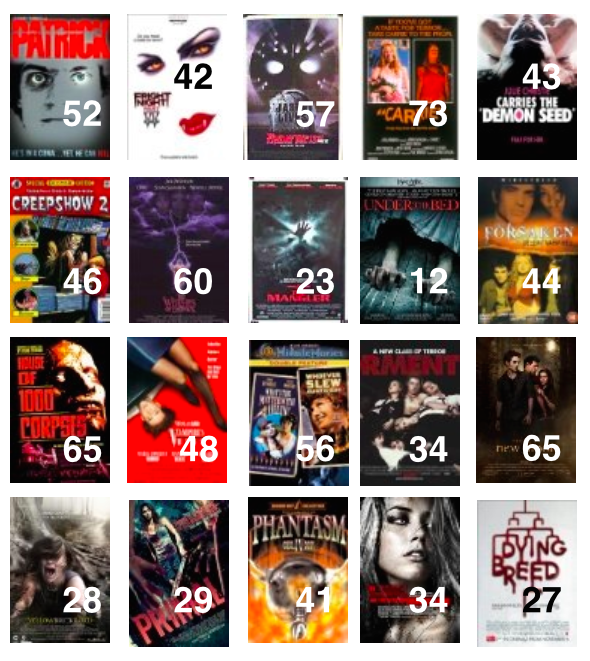
\includegraphics[width = \textwidth]{figures/movies/horror_data}
}

\end{frame}

%%%%%%%%%%%%%%%%%%%%%%%%%%%%%%%%%%%

\begin{frame}[fragile]
\frametitle{Data}

{\scriptsize
\begin{verbatim}
                                  title audience_score
 1                              Patrick             52
 2                           Demon Seed             43
 3                            Tormented             34
 4                        Under the Bed             12
 5                Phantasm IV: Oblivion             41
 6                  Fright Night Part 2             42
 7                House of 1000 Corpses             65
 8                          Creepshow 2             46
 9                         The Forsaken             44
10         All the Boys Love Mandy Lane             34
11 Jason Lives: Friday the 13th Part VI             57
12                       Vampire's Kiss             48
13              The Witches of Eastwick             60
14                      Yellowbrickroad             28
15                          Dying Breed             27
16                               Carrie             73
17             Whoever Slew Auntie Roo?             56
18                          The Mangler             23
19                               Primal             29
20          The Twilight Saga: New Moon             65
\end{verbatim}
}

\end{frame}

%%%%%%%%%%%%%%%%%%%%%%%%%%%%%%%%%%%

\begin{frame}
\frametitle{First look}

\disc{{\small The histogram below shows the distribution of the audience scores of these movies 
(ranging from 0 to 100). The median score in the sample is 43.5. Can we apply CLT based methods 
we have learned so far to construct a confidence interval for the \underline{median} RottenTomatoes 
score of horror movies. Why or why not?}}

\begin{center}
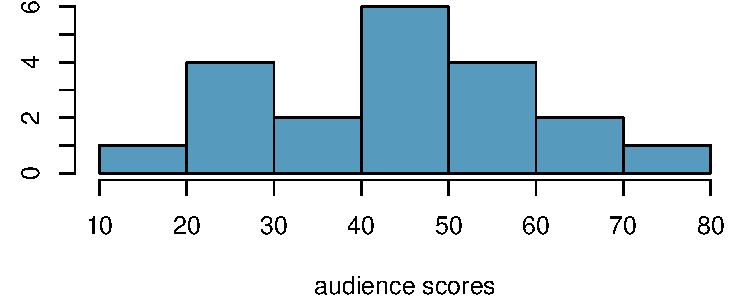
\includegraphics[width = 0.8\textwidth]{figures/movies/horror_hist}
\end{center}

\end{frame}

%%%%%%%%%%%%%%%%%%%%%%%%%%%%%%%%%%%

\begin{frame}
\frametitle{Bootstrapping}

\begin{itemize}

\item An alternative approach to constructing confidence intervals is \hl{bootstrapping}. 

\pause

\item This term comes from the phrase ``pulling oneself up by one's bootstraps", which is a metaphor 
for accomplishing an impossible task without any outside help. 

\pause

\item In this case the \sout{im}possible task is estimating a population parameter, and we'll accomplish 
it using data from only the given sample.

\end{itemize}

\hfill 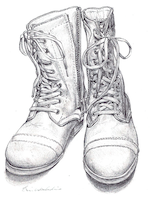
\includegraphics[width = 0.25\textwidth]{figures/boot}

\end{frame}

%%%%%%%%%%%%%%%%%%%%%%%%%%%%%%%%%%%%%

\begin{frame}
\frametitle{Bootstrapping}

\begin{itemize}

\item Bootstrapping works as follows:
\pause
\begin{enumerate}[(1)]
\item take a bootstrap sample - a random sample taken with replacement from the original sample, of the 
same size as the original sample
\pause
\item calculate the bootstrap statistic - a statistic such as mean, median, proportion, etc. computed on the 
bootstrap samples
\pause
\item repeat steps (1) and (2) many times to create a bootstrap distribution - a distribution of bootstrap statistics
\end{enumerate}

\pause

\item The XX\% bootstrap confidence interval can be estimated by
\begin{itemize}
\pause
\item the cutoff values for the middle XX\% of the bootstrap distribution,
\item[]
\pause
\item[] OR
\item[]
\pause
\item $point~estimate \pm t^\star SE_{boot}$
\end{itemize}

\end{itemize}

\end{frame}

%%%%%%%%%%%%%%%%%%%%%%%%%%%%%%%%%%%%%

\begin{frame}[fragile]
\frametitle{Bootstrap sample 1}

{\small \textbf{(1) Take a bootstrap sample:}}
\pause
{\tiny
\begin{verbatim}
                                  title audience_score
 1                       Vampire's Kiss             48
 2                Phantasm IV: Oblivion             41
 3                House of 1000 Corpses             65
 4                          Dying Breed             27
 5             Whoever Slew Auntie Roo?             56
 6                         The Forsaken             44
 7          The Twilight Saga: New Moon             65
 8          The Twilight Saga: New Moon             65
 9             Whoever Slew Auntie Roo?             56
10          The Twilight Saga: New Moon             65
11                          The Mangler             23
12                          Dying Breed             27
13                          Creepshow 2             46
14                House of 1000 Corpses             65
15             Whoever Slew Auntie Roo?             56
16                            Tormented             34
17 Jason Lives: Friday the 13th Part VI             57
18                       Vampire's Kiss             48
19                               Primal             29
20              The Witches of Eastwick             60
\end{verbatim}
}

\pause

{\small \textbf{(2) Calculate the median of the bootstrap sample:}} \\
\pause
{\footnotesize
23, 27, 27, 29, 34, 41, 44, 46, 48, \red{48, 56}, 56, 56, 57, 60, 65, 65, 65, 65, 65 \\
median = (48 + 56) / 2 = 52 \\
}

\pause

{\small
\textbf{(3) Record this value}
}

\end{frame}

%%%%%%%%%%%%%%%%%%%%%%%%%%%%%%%%%%%%%

\begin{frame}[fragile]
\frametitle{Bootstrap sample 2}

{\small \textbf{(1) Take another bootstrap sample:}}
\pause
{\tiny
\begin{verbatim}
                                  title audience_score
 1                  Fright Night Part 2             42
 2                               Carrie             73
 3                         The Forsaken             44
 4                          The Mangler             23
 5                               Primal             29
 6                              Patrick             52
 7 Jason Lives: Friday the 13th Part VI             57
 8                          The Mangler             23
 9                       Vampire's Kiss             48
10         All the Boys Love Mandy Lane             34
11          The Twilight Saga: New Moon             65
12         All the Boys Love Mandy Lane             34
13                      Yellowbrickroad             28
14                       Vampire's Kiss             48
15                            Tormented             34
16                          The Mangler             23
17                Phantasm IV: Oblivion             41
18                              Patrick             52
19                House of 1000 Corpses             65
20          The Twilight Saga: New Moon             65
\end{verbatim}
}

\pause

{\small \textbf{(2) Calculate the median of the bootstrap sample:}} \\
\pause
{\footnotesize
23, 23, 23, 28, 29, 34, 34, 34, 41, \red{42, 44}, 48, 48, 52, 52, 57, 65, 65, 65, 73 \\
median = (42 + 44) / 2 = 43 \\
}

\pause

{\small
\textbf{(3) Record this value}
}

\end{frame}

%%%%%%%%%%%%%%%%%%%%%%%%%%%%%%%%%%%%%

\begin{frame}[fragile]
\frametitle{Bootstrap sample 3}

{\small \textbf{(1) Take another bootstrap sample:}}
\pause
{\tiny
\begin{verbatim}
                                  title audience_score
 1                            Tormented             34
 2              The Witches of Eastwick             60
 3              The Witches of Eastwick             60
 4              The Witches of Eastwick             60
 5                          The Mangler             23
 6              The Witches of Eastwick             60
 7                              Patrick             52
 8                Phantasm IV: Oblivion             41
 9                      Yellowbrickroad             28
10 Jason Lives: Friday the 13th Part VI             57
11                      Yellowbrickroad             28
12 Jason Lives: Friday the 13th Part VI             57
13                  Fright Night Part 2             42
14                               Primal             29
15                  Fright Night Part 2             42
16             Whoever Slew Auntie Roo?             56
17                  Fright Night Part 2             42
18                  Fright Night Part 2             42
19                        Under the Bed             12
20                Phantasm IV: Oblivion             41
\end{verbatim}
}

\pause

{\small \textbf{(2) Calculate the median of the bootstrap sample:}} \\
\pause
{\footnotesize
12, 23, 28, 28, 29, 34, 41, 41, 42, \red{42, 42}, 42, 52, 56, 57, 57, 60, 60, 60, 60 \\
median = (42 + 42) / 2 = 42 \\
}

\pause

{\small
\textbf{(3) Record this value}
}

\end{frame}

%%%%%%%%%%%%%%%%%%%%%%%%%%%%%%%%%%%%%

\begin{frame}
\frametitle{Many more bootstrap samples}

\vfill

... repeat

\vfill

\end{frame}

%%%%%%%%%%%%%%%%%%%%%%%%%%%%%%%%%%%%%

\begin{frame}
\frametitle{}

\clicker{The dot plot  below is the bootstrap distribution of medians constructed using 100 simulations. 
What does each dot on the dot plot represent?}

\begin{center}
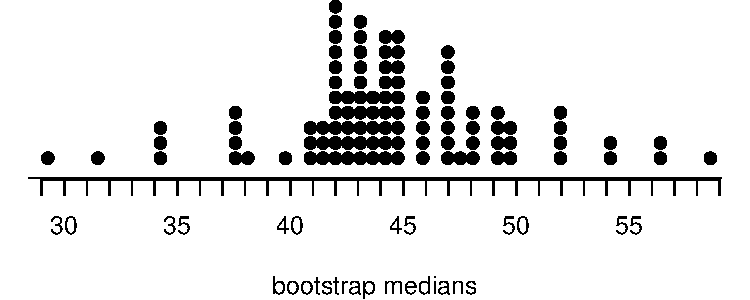
\includegraphics[width = 0.6\textwidth]{figures/movies/horror_boot_med_dot}
\end{center}

\begin{enumerate}[(a)]
\item Score of a horror movie in the original sample
\item Score of a horror movie in the population
\item \solnMult{Median from one bootstrap sample from the original sample}
\item Median from one sample from the population
\end{enumerate}

\end{frame}

%%%%%%%%%%%%%%%%%%%%%%%%%%%%%%%%%%

\subsection{Bootstrap percentile intervals: middle XX\% of the bootstrap distribution}
\label{mi2}

%%%%%%%%%%%%%%%%%%%%%%%%%%%%%%%%%%

\begin{frame}
\frametitle{}

\clicker{The dot plot  below shows the distribution of 100 bootstrap medians. Estimate the 90\% bootstrap 
confidence interval for the median RT score of horror movies using the percentile method.}

\only<1>{
\begin{center}
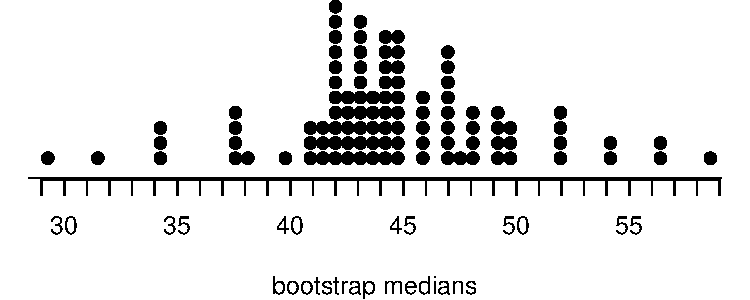
\includegraphics[width = 0.8\textwidth]{figures/movies/horror_boot_med_dot}
\end{center}
}

\soln{\only<2->{
\begin{center}
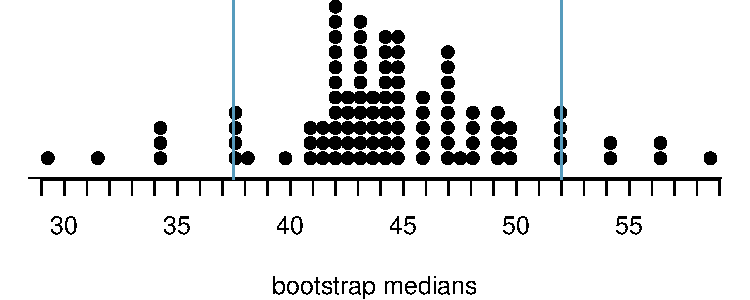
\includegraphics[width = 0.8\textwidth]{figures/movies/horror_boot_med_dot_soln}
\end{center}
}}

\begin{multicols}{2}
\begin{enumerate}[(a)]
\item (29, 58.5)
\item (34, 57)
\item \solnMult{(37.5, 52)}
\item (40, 49.5)
\end{enumerate}
\end{multicols}

\end{frame}

%%%%%%%%%%%%%%%%%%%%%%%%%%%%%%%%%

\subsection{Bootstrap SE intervals: point estimate $\pm$ ME}
\label{mi3}

%%%%%%%%%%%%%%%%%%%%%%%%%%%%%%%%%

\begin{frame}
\frametitle{Bootstrap interval, standard error}

\disc{The dot plot  below shows the distribution of 100 bootstrap medians. The median of the original 
sample is 43.5 and the bootstrap standard error is 4.88. Estimate the 90\% bootstrap confidence interval 
for the median RT score of horror movies using the standard error method.}

\twocol{0.50}{0.50}{
\begin{center}
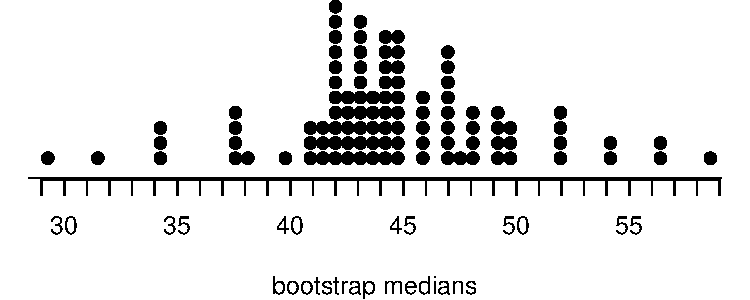
\includegraphics[width = \textwidth]{figures/movies/horror_boot_med_dot}
\end{center}
}
{
\pause
\begin{center}
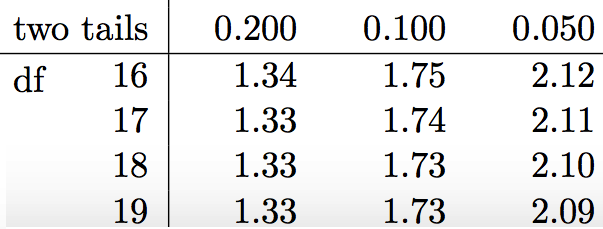
\includegraphics[width = \textwidth]{figures/movies/t_19}
\end{center}
}

\soln{\[ 43.5 \pm (1.73 \times 4.88) = (35.1, 51.9) \] }

\end{frame}

%%%%%%%%%%%%%%%%%%%%%%%%%%%%%%%%%

\begin{frame}
\frametitle{Bootstrap vs. sampling distributions}

\vfill

\app{4.2 Bootstrap intervals}{See the course webpage for details.}

\vfill

\end{frame}

%%%%%%%%%%%%%%%%%%%%%%%%%%%%%%%%%%

\subsection{Bootstrap testing for a single numerical variable requires shifting the
bootstrap distribution to be centered at the null value}
\label{mi4}

%%%%%%%%%%%%%%%%%%%%%%%%%%%%%%%%%%%

\begin{frame}
\frametitle{Bootstrap testing for a mean}

\begin{itemize}

\item This is very similar to bootstrapping, i.e. we randomly sample with replacement from the sample, 
but this time we shift the bootstrap distribution to be \underline{centered at the null value}. 

\pause

\item The p-value is then defined as the proportion of simulations that yield a sample statistic at least as 
favorable to the alternative hypothesis as the observed sample statistic.

\end{itemize}

\end{frame}

%%%%%%%%%%%%%%%%%%%%%%%%%%%%%%%%%%%

\begin{frame}
\frametitle{}

\disc{Do these data provide convincing evidence that the median audience score of horror movies is greater 
than 40? Remember that the median of the original sample was 43.5.}

\begin{center}
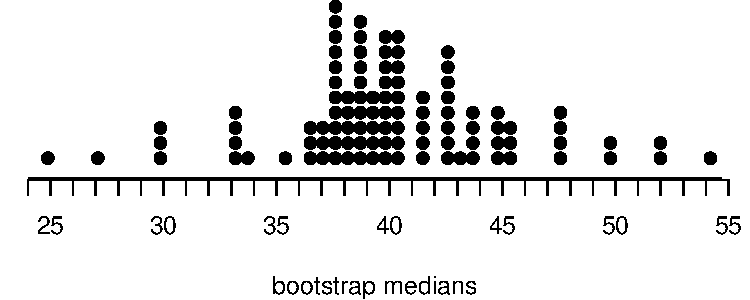
\includegraphics[width = 0.75\textwidth]{figures/movies/horror_boot_med_test_dot}
\end{center}

\pause

\twocol{0.3}{0.7}{
\begin{itemize}
\item[$H_0:$] $median = 40$
\item[$H_A:$] $median > 40$
\end{itemize}
}
{
\pause
p-value: proportion of simulations where the simulated bootstrap sample median is at least as extreme as the 
one observed (43.5). $\rightarrow$ 20 / 100 = 0.20
}

\end{frame}

%%%%%%%%%%%%%%%%%%%%%%%%%%%%%%%%%%%

\section{Summary}

%%%%%%%%%%%%%%%%%%%%%%%%%%%%%%%%%%%

\begin{frame}
\frametitle{Summary of main ideas}

\vfill

\begin{enumerate}

\item \nameref{mi1}

\item \nameref{mi2}

\item \nameref{mi3}

\item \nameref{mi4}

\end{enumerate}

\vfill

\end{frame}

%%%%%%%%%%%%%%%%%%%%%%%%%%%%%%%%%%%

\end{document}